\subsection{Hypergraphen}
Hypergraphen stellen eine Generalisierung von Graphen dar und ermöglichen die Modelierung komplexer Beziehungen \cite{anglesintro}.
%Hypergraphen haben die Eigenschaft, dass Kanten im Gegensatz zu klassischen Graphen mehr als zwei Knoten miteinander verbinden können.
%Die Kanten des Hypergraphen werden auch als Hyperkanten bezeichnet.
Im Vergleich zum normalen Graphen können die Kanten eines Hypergraphen eine beliebige Kardinalität haben.
Die Hyperedges in einem Hypergraphen verbinden somit eine beliebige Menge von Knoten, was eine direkte Darstellung von Beziehungen höherer Ordnung ermöglicht \cite{iordanov2010hypergraphdb}.
Im Falle eines gerichteten Hypergraphen verbindet die Hyperkante den Ausgangsknoten direkt mit allen Zielknoten.
%\\Mathematisch ist ein Hypergraph folgendermaßen definiert:
%\begin{definition}
%	Let $X=\{v_{1}, v_{2},...,v_{n}\}$ be a finite set,
%	and let $E=\{e_{1},e_{2},...,e_{m}\}$ be a family of subsets of $X$ such that
%	\[e_{i} \neq \varnothing (i=1,2,...,m) \\
%	\cup_{i=1}^{m}e_{i}=X.
%	\]
%	The pair $H=(X,E)$ is called a hypergraph with vertex set $X$
%	and hyperedge set $E$. The elements $v_{1}, v_{2},...,v_{n}$ of $X$ are vertices
%	of hypergraph $H$, and the sets $e_{1}, e_{2},...,e_{m}$ are hyperedges of hypergraph $H$ \cite[Seite 2]{zhang2018hypergraph}.
%\end{definition}

Abbildung \ref{2.hyper.image} zeigt einen Hypergraphen.
Die Kante $e_{4}$ verbindet in diesem Graphen die Knoten $v_{5}$, $v_{6}$ und $v_{7}$ miteinander.
\begin{figure}[H]
\begin{center}
	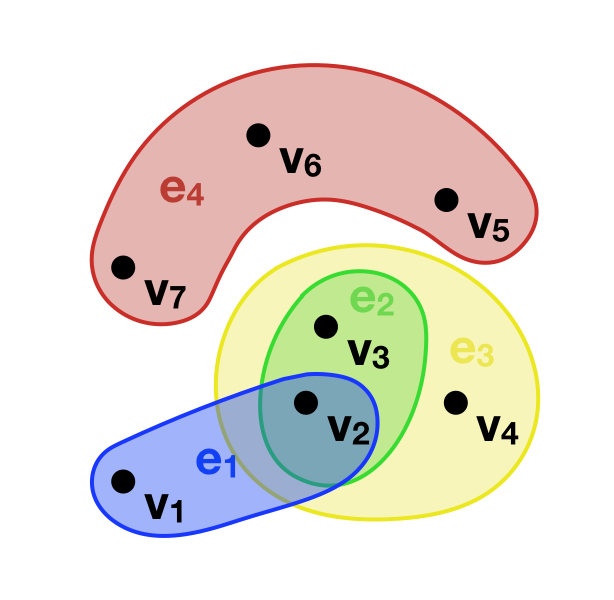
\includegraphics[scale = 0.5]{./images/Hypergraph2.png}
	\label{2.hyper.image}
	\caption{Hypergraph}
\end{center}
\end{figure}
%Hypergraphen ermöglichen die direkte Darstellung rekursiver Beziehungen \cite{iordanov2010hypergraphdb}.
Da Hypergraphen die direkte Darstellung rekursiver Beziehungen ermöglichen und somit eine flexiblere Struktur als das einfache Graphen-Modell bieten, werden diese oft zur Modellierung in Graphdatenbanken verwendet \cite{iordanov2010hypergraphdb}\cite{flockdb}.
Eine Datenbank, die Hypergraphen als Datenbankmodell nutzt ist beispielsweise HyperGraphDB, welche von Kobrix Software Inc entwickelt wurde \cite{iordanov2010hypergraphdb}.
Ein weiteres Projekt, bei dem Hypergraphen zur Modellierung genutzt werden ist Trinity \cite{shao2013trinity}.
%In einem normale Graphen sind die Kanten, eine in einem Intervall festgelegte Menge von Knoten:
%    \[X = \{v_{1}, v_{2}, v_{3}, v_{4}, v_{5}, v_{6}, v_{7}\} \text{ Knoten}\]
%    \[E=\{e_{1}, e_{2}, e_{3}, e_{4}\} \text{ Kanten}\]
%    \[E=\{e_{1}, e_{2}, e_{3}, e_{4}\} = \{\{v_{1}, v_{2}, v_{3}\}, \{v_{2}, v_{3}\}, \{v_{3}, v_{5}, v_{6}\}, \{v_{4}\}\} \]
%Transversals
%\subsection{Multimodale Graphen}
%\subsection{Hypertree}
%\subsection{k-uniform hypergraph}
